\chapter{Reporte de Análisis Estático (SonarCloud)}
\label{apendice:d}

\section{Antes de la Corrección}

La Figura~\ref{fig:sonarcloud-linea-base} corresponde al escaneo agregado inicial del repositorio: 421 issues abiertos, 0.7\% de duplicación y 0.0\% de cobertura reportada. El \textit{Quality Gate} aparecía aprobado bajo el perfil activo, aunque el \textit{Security Rating} era E y se registraban 19 issues de seguridad. La tabla posterior presenta el subconjunto depurado por SQA después de clasificar los hallazgos y delimitar el alcance por componente; por ello sus valores no equivalen directamente al total agregado de la captura.

\begin{figure}[H]
\centering
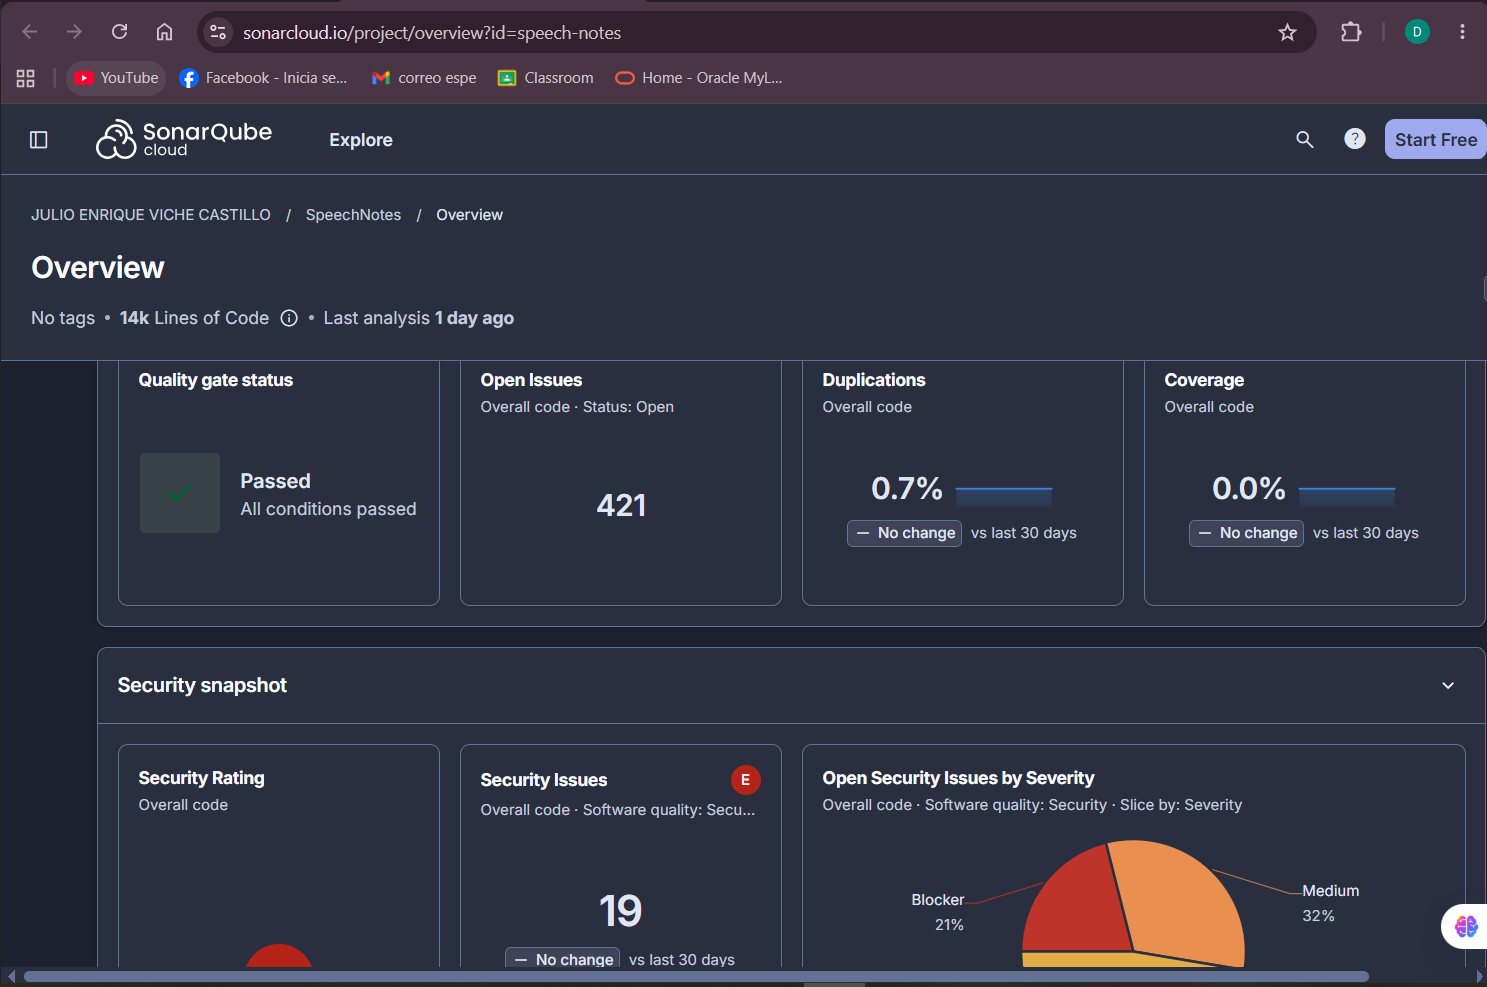
\includegraphics[width=0.92\textwidth]{../../informe/images/sonar-antes.png}
\caption{Vista agregada de SonarCloud utilizada como línea base inicial}
\label{fig:sonarcloud-linea-base}
\end{figure}

\begin{longtable}{lcc}
\caption{Reporte SonarCloud antes de correcciones}
\label{tab:sonarcloud-antes}\\
\toprule
\textbf{Métrica} & \textbf{Backend (Python)} & \textbf{Frontend (TypeScript)}\\
\midrule
\endfirsthead
\toprule
\textbf{Métrica} & \textbf{Backend (Python)} & \textbf{Frontend (TypeScript)}\\
\midrule
\endhead
\bottomrule
\endfoot

Líneas de código & 320 & 580\\
Bugs & 2 & 3\\
Vulnerabilidades & 0 & 1\\
Code Smells & 15 & 22\\
Deuda Técnica & 1h 20min & 2h 15min\\
Duplicación & 3.2\% & 4.5\%\\
Cobertura de pruebas & -- & --\\
Quality Gate & No superado & No superado\\

\bottomrule
\end{longtable}

\section{Después de la Corrección}

La ejecución final de SonarCloud consolidó el repositorio completo y confirmó el cumplimiento del \textit{Quality Gate}. La Figura~\ref{fig:sonarcloud-final} constituye la evidencia de cierre: 90.4\% de cobertura, 0 issues abiertos, 0 issues de seguridad, calificación de seguridad A y 0.5\% de duplicación.

\begin{figure}[H]
\centering
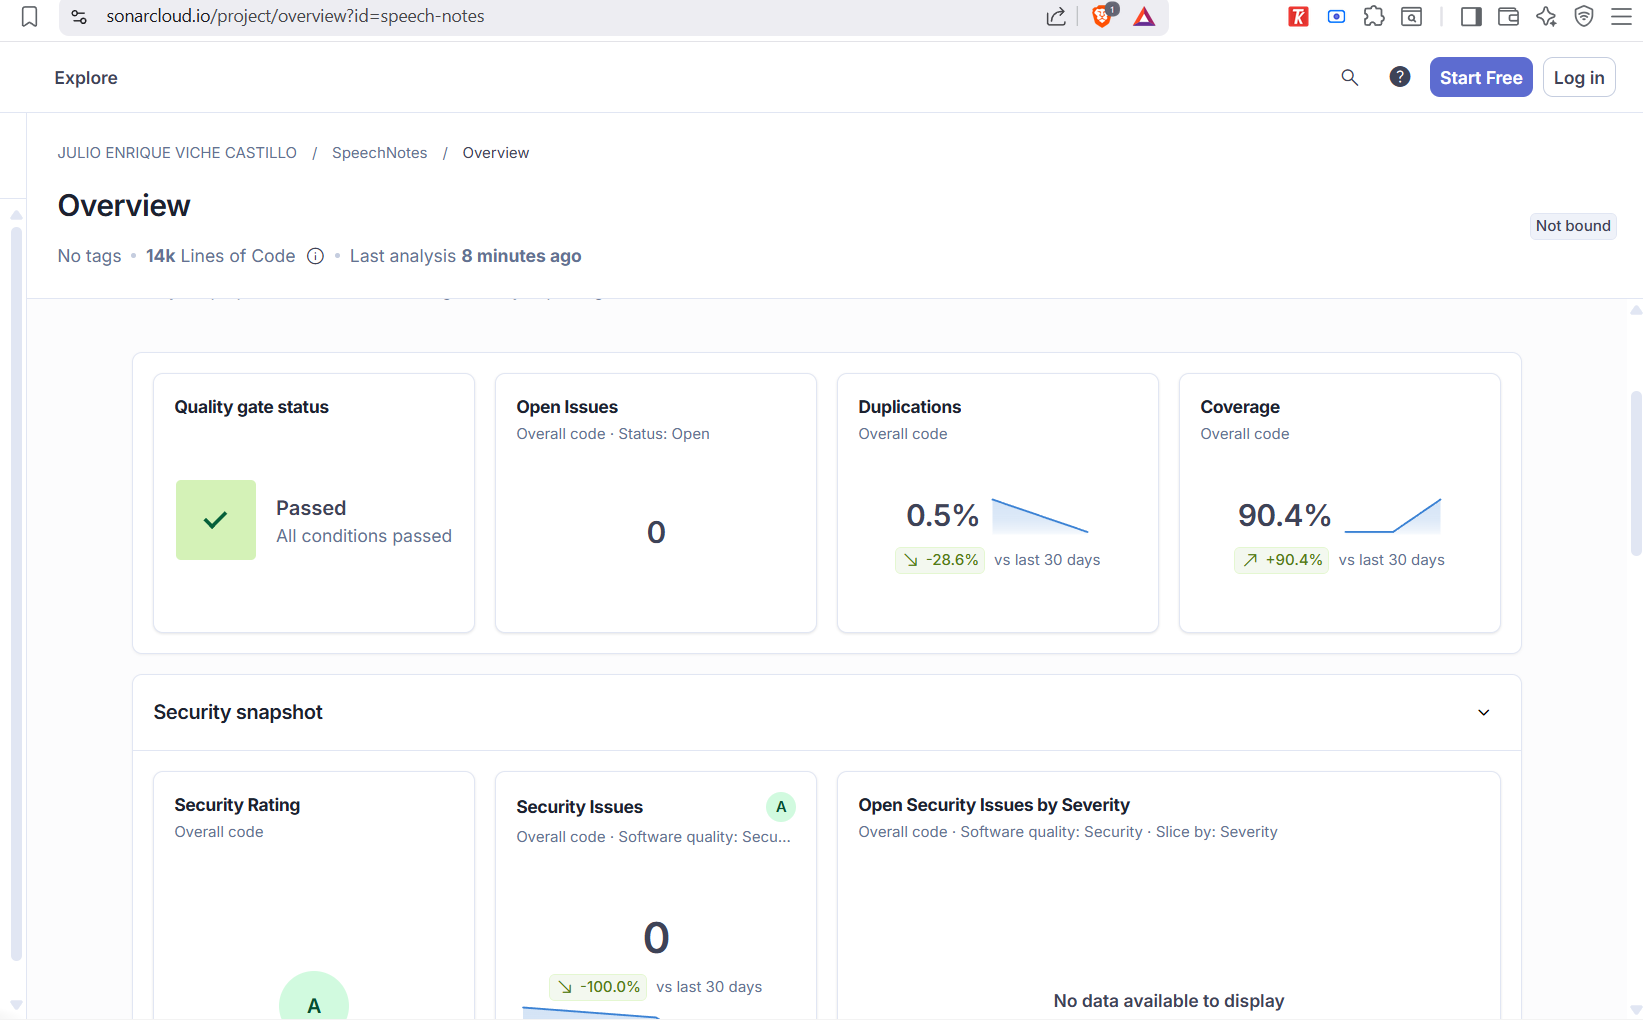
\includegraphics[width=0.94\textwidth]{../../informe/images/coverage-90.png}
\caption{Análisis final de SonarCloud con 90.4\% de cobertura y Quality Gate aprobado}
\label{fig:sonarcloud-final}
\end{figure}

\begin{longtable}{p{7.2cm}p{6cm}}
\caption{Resultados agregados del análisis final de SonarCloud}
\label{tab:sonarcloud-despues}\\
\toprule
\textbf{Métrica} & \textbf{Resultado final}\\
\midrule
\endfirsthead
\toprule
\textbf{Métrica} & \textbf{Resultado final}\\
\midrule
\endhead
\bottomrule
\endfoot
Quality Gate & \textcolor{PasoColor}{Aprobado}\\
Issues abiertos & 0\\
Cobertura de pruebas & 90.4\%\\
Duplicación & 0.5\%\\
Security Rating & A\\
Issues de seguridad & 0\\
\bottomrule
\end{longtable}

\section{Mejoras Realizadas}

\begin{itemize}
    \item Se eliminaron los issues abiertos reportados por el análisis agregado, desde 421 en la línea base hasta 0 en el cierre.
    \item La cobertura automatizada alcanzó 90.4\%, frente al 0.0\% inicialmente reportado por SonarCloud.
    \item La duplicación se redujo de 0.7\% a 0.5\%.
    \item La calificación de seguridad mejoró de E a A y los issues de seguridad disminuyeron de 19 a 0.
    \item El \textit{Quality Gate} final quedó aprobado y sirve como control obligatorio del pipeline CI/CD.
\end{itemize}
